\chapter{Architektur}
Nachdem wir unser Projektziel für uns gesetzt hatten, mussten wir schauen wie das sich realisieren lässt. Als erstes einigten wir uns darauf das wir einen Raspberry Pi für die externe Zugsteuerung benutzen. Dann mussten wir uns überlegen wie wir den Zug mit dem Raspberry Pi kommunizieren lassen, damit diese Informationen zwischen einander austauschen können. Bevor wir das aber entscheiden konnten mussten wir uns erst Gedanken darüber machen welche Aufgaben der Raspbery Pi und der Zug haben.

Zuerst haben wir uns überlegt was der Zug alles können muss, was grob gesagt nur das transportieren von Fahrgästen von Bahnhof zu Bahnhof ist. Daraus konnten wir schnell ableiten das die Erkennung seiner aktuellen Position eine der wichtigsten Aufgaben des Zugs ist, denn wenn wir nicht wissen wo der Zug ist, dann können wir ihm auch nicht sagen wo er hinfahren soll. Des weiteren muss der Zug einstellen können wie schnell er fährt und Information übermitteln können. Damit hatten wir die ungefähre Funktionalität des Zuges bestimmt und konnten uns dem Raspberry Pi zuwenden. Dieser muss als eine externe Steuereinheit bestimmen welchen Weg der Zug fahren soll. Dazu braucht er die Informationen wo sich der Zug befindet und an welchem Bahnhof Personen stehen und wohin diese gehen wollen. Des weiteren muss er dann noch dem Zug übermitteln können wohin er als nächstes fahren soll. Mit unseren Überlegungen hatten wir schon automatisch unsere Frage zur Kommunikation beantwortet. Denn der Zug muss dem Raspberry Pi seine aktuelle Position übermitteln und der Raspberry Pi muss dem Zug einen Befehl schicken wohin und mit welcher Geschwindigkeit er als nächstes fahren soll. 

Nachdem wir unsere Fragen beantwortet hatten, wollten wir versuchen diese mit Hilfe eines Klassendiagramms zu konkretisieren (Siehe Abbildung \ref{pic:ClassDiagram}).In nachfolgenden sind alle Klassen die Thread in ihrem Namen haben auch Threads. Die Klasse LocateThread in der Train-Komponente des Klassendiagramms beschäftigt sich ausschließlich mit der Bestimmung der Position des Zuges. Zur Bestimmung der Position  haben wir auf der Strecke RFID-Tags verteilt die der LocateThread vom Zug beim Überfahren lesen kann und danach sie weiter an die Klasse TrainSpeakerThread schickt. Dieser vergleicht nach erhalten der Position diese mit der eingetragenen Position in der Klasse Order. Falls die Positionen sich unterscheiden ist entweder etwas schiefgelaufen oder der Zug ist gerade erst angefahren und hat zum ersten mal seine Position bestimmt. Bei beiden Fällen wird die Geschwindigkeit des Zugs auf 0 gesetzt und er wartet somit auf weitere Befehle. Falls die Positionen gleich sind wird die afterSpeed Geschwindigkeit aus der Klasse Order genommen und dem TrainThread übermittel, welcher dann diese Geschwindigkeit setzt. Als letztes schickt der TrainSpeakerThread über eine Socket-Verbindung die Position des Zuges an den Raspberry Pi. Diese Nachricht kommt dann an die Klasse PiListenerThread, welcher diese in der Klasse TrainStatus abspeichert. Danach kann die Klasse PiAlgorithm, welche auch ein Thread ist, die aktuelle Position des Zugs aus dem TrainStatus auslesen und schauen wohin der Zug als nächstes fahren soll(genaueres wird im Kapitel Algorithm erklärt). Diesen Befehl schickt er an den PiSpeakerThread, welcher diesen weiter über die Socket-Verbindung schickt. Der Befehl wird vom TrainListenerThread erhalten, welcher den Befehl in der Klasse Order speichert. Zuletzt wird noch die beforeSpeed Geschwindigkeit die im Befehl enthalten ist an den TrainThread übermittelt, welcher dann die Geschwindigkeit des Zuges darauf setzt. Damit hätte man einen gesamten Durchlauf gemacht, welcher wieder von neuen beginnt wenn der Zug eine neue Position liest.  


\begin{figure}[H]	
\caption{Klassendiagramm}
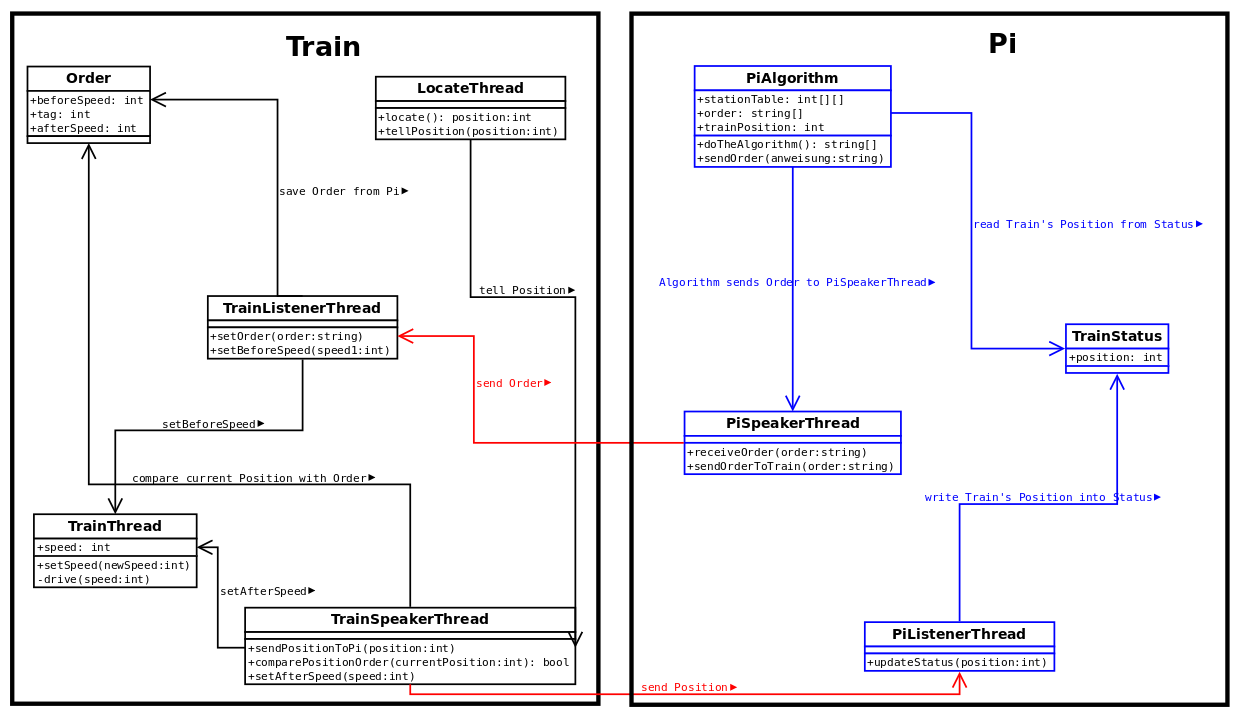
\includegraphics[width=2\textwidth, width=465pt]{content/images/ClassDiagram.png}
\label{pic:ClassDiagram}
\end{figure}



\begin{figure}[H]	
\caption{Use Case Diagramm}
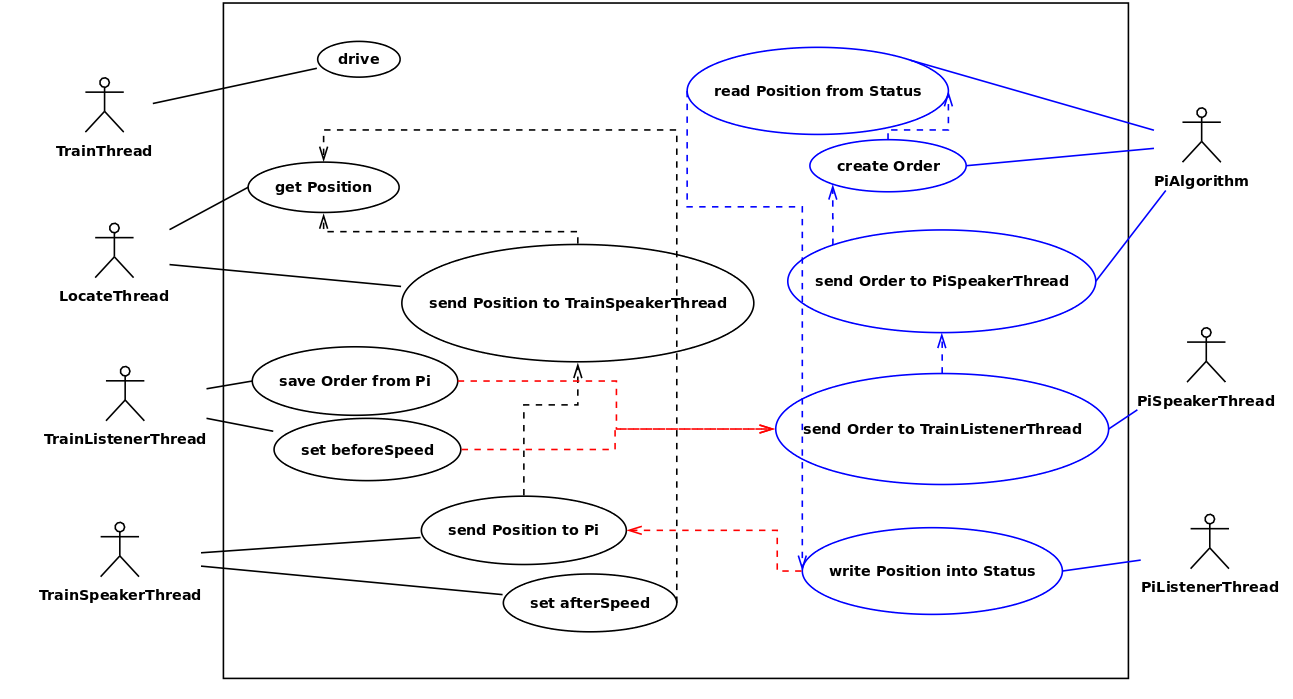
\includegraphics[width=2\textwidth, width=465pt]{content/images/UseCaseDia.png}
\label{pic:UseCaseDiagram}
\end{figure}
